% !TeX spellcheck = es_ES
% !TeX root = ../metalurgy.tex
\part{Curvas de transformación tiempo-temperatura (TTT) y CCT}
Tambien conocidos como diagramas de transformación isotérmica, son tres aspectos los que dominan estas curvas:
\begin{itemize}
    \item Tiempo: Una vez que la temperatura de la austenita baja por debajo de \Aone se vuelve inestable y comienza a transformarse con el tiempo. 
    \item Morfología: Distribución, tamaño y forma de los productos obtenidos a partir de su transformación. son clave para las propiedades que se obtienen.
    \item Fases que no están en equilibrio: La aparición de fases fuera de equilibrio, como por ejemplo, la martensita
\end{itemize}
Los CCT son \textit{Continuous Cooling transformation} para enfriamiento a $\frac{\partial T}{\partial t}= \text{constante}$.


\begin{figure}[ht]
    \centering
    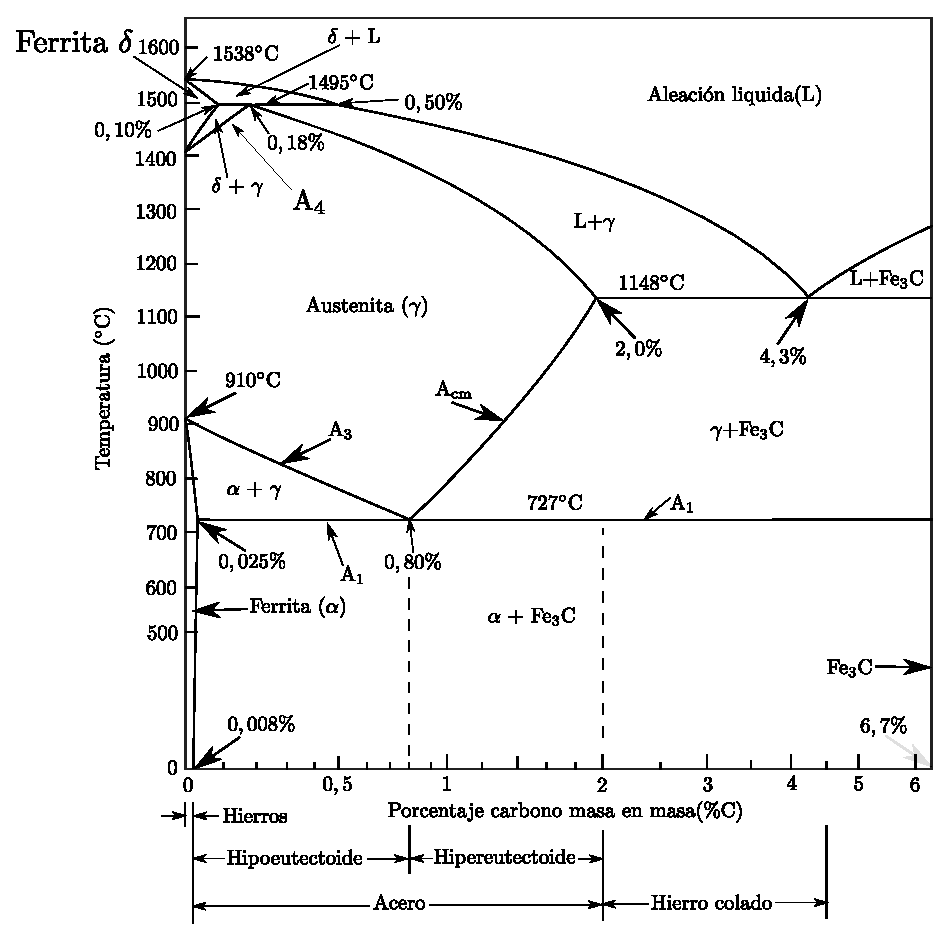
\includegraphics[width=1\textwidth]{fig/diagAceroreal.eps}
    \caption{Diagramas de fases para aceros.}
    \label{fig:diagAceros}
\end{figure}

Fases
\begin{itemize}
    \item Perlita: Morfología laminar, su transformación se favorece con mayor coeficiente de difusión.
    \item Bainita: Morfología con $\alpha$ en listones y carburos discretos
    \item Martensita: Misma composición que austenita pero red cristalina diferente (BCT) y distorsionada. Contiene zonas de austenita.
\end{itemize}



\section{Acero eutectoide}
Se comienza estudiando las transformaciones isotérmicas de la austenita
\begin{figure}[htb!]
    \centering
    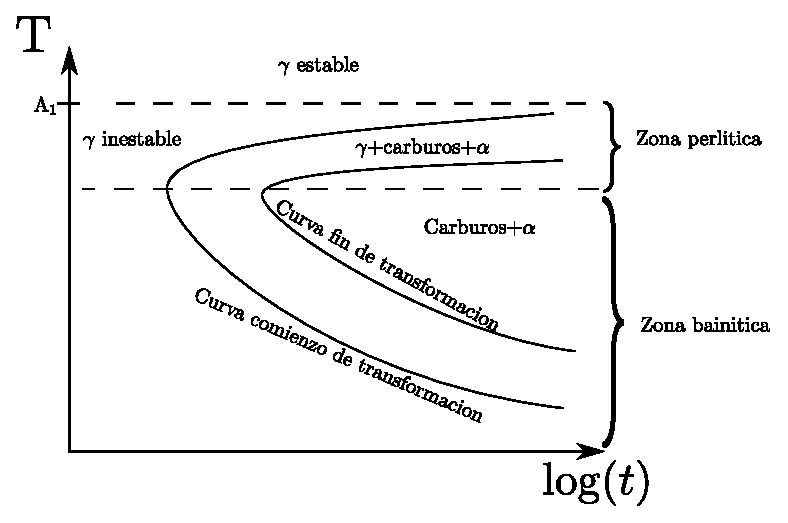
\includegraphics[width=\textwidth]{fig/TTTbasic.eps}
    \caption{Diagrama para transformación isotérmica de la austenita para un acero \textbf{eutectoide}.}
    \label{fig:diagTTTbasico}
\end{figure}

\begin{figure}[htb!]
    \centering
    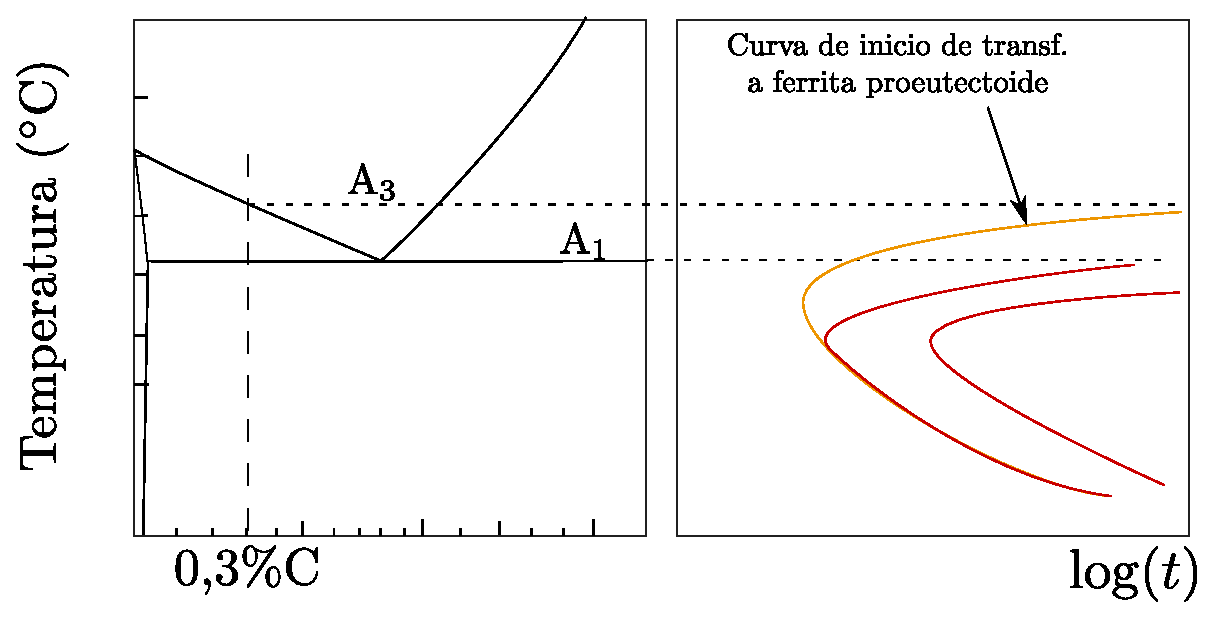
\includegraphics[width=\textwidth]{fig/diagTTThipo.eps}
    \caption{Diagrama para transformación isotérmica de la austenita para un acero \textbf{hipoeutectoide} (0,3\%).}
    \label{fig:diagTTThipo}
\end{figure}

\begin{figure}[htb!]
    \centering
    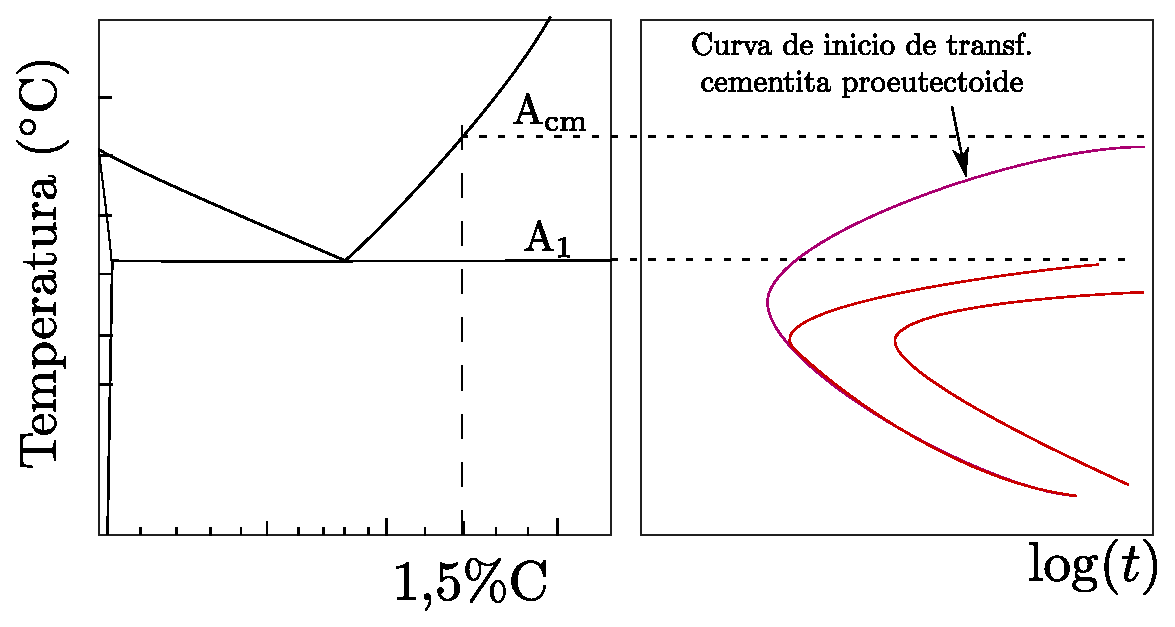
\includegraphics[width=\textwidth]{fig/diagTTThiper.eps}
    \caption{Diagrama para transformación isotérmica de la austenita para un acero \textbf{hipereutectoide} (1,5\%).}
    \label{fig:diagTTThiper}
\end{figure}

La nariz de la figura \ref{fig:diagTTTbasico} se da porque hay competencia entre la \textbf{fuerza impulsora} $\Delta G$ (dominante a bajas temperaturas) y el \textbf{coeficiente de difusión de carbono} $D_c$ (aumenta con temperatura).

Transformación perlítica



\section{Competencia entre G y D}
A temperaturas cercanas a \Aone la difusión domina mientras que a bajas temperaturas hay alta fuerza impulsora debido a que la inestabilidad de la austenita. Hay una temperatura a la cual se complementan y la transformación tiene una velocidad máxima, en la figura \ref{fig:diagTTTbasico} seria la nariz (450 a 600 \grad).

\section{Microconstituyentes}
Los productos de transformación de la austenita que combinan
ferrita y carburos de Fe, así como las fases proeutectoides, se denominan genéricamente \textbf{microconstituyentes} para diferenciarlos de las verdaderas fases que los componen.
\begin{itemize}
    \item Si enfriamos justo por debajo de \Aone~ la fuerza impulsora va ser baja  y van a prevalecer los sitios de nucleacion preferencial (bordes de grano). Comienza a nuclear a la par la ferrita y la cementita cooperativamente formando un microconstituyente con morfologia laminar denominado \textbf{perlita}. Ocurre por arriba de la nariz para subenfriamientos bajos ($<170\grad$).
    \item En cambio, en el rango de temperaturas por debajo de la nariz la ferrita nuclea primero, adopta una morfología de listones, y los carburos ya no son laminares sino discretos con forma de placas más o menos cortas. Por otra parte la transformación en esta zona tiene un mecanismo diferente al aquel que ocurre a altas temperaturas. Los microconstituyentes obtenidos en esta zona se denominan genéricamente \textbf{bainitas} y los hay de varios tipos.
    \item Finalmente, a temperaturas muy bajas ($<$ 350\grad) la austenita subenfriada transforma anisotérmicamente y sin difusión a una fase metaestable denominada martensita.
\end{itemize}


\section{Perlita}
Para generar perlita se requiere un alto coeficiente de difusión de carbono ya que se están generando zonas de muy bajo carbono (ferrita $\alpha$) y zonas de alto carbono (cementita $\cementita$) lo que requiere mucha difusión partiendo de austenita ($\gamma$). Prevalecen los sitios de nucleación preferencial debido a la baja fuerza impulsora $\Delta G$.

El \textbf{espaciado interlaminar} $S$ es el principal parámetro geométrico de la perlita. Tiene gran importancia y determina muchas propiedades. Es la distancia entre laminas contiguas de la misma fase medida perpendicularmente al eje longitudinal de las laminas (básicamente miras la foto de microscopio de electrones y ves cuanto espacio hay entre comienzos de dos laminas de cementita/ferrita). Existe la perlita gruesa ($S\approx 1\si{\micro \meter}$) y perlita fina $S< 0,3\si{\micro \meter}$. A mayor subenfriado menor es $D_c$, menos se puede desplazar el carbono y por ende menor va ser la distancia entre laminas de \cementita~ y $\alpha$.
\begin{equation}\label{eq:StoPerliteStrength}
    R_{p 0,2}, R_{m}, H V \propto S^{-\frac{1}{2}}
\end{equation}

Perlita mas fina trae dureza, resistencia y mayor tensión de fluencia. A su vez es mas difícil de formar, mecanizar etc.

\section{Transformación Martensita}
Cuando la austenita se sobrenfría hasta temperaturas muy bajas se produce una transformación sin difusión de C donde, en un volumen discreto de material, los átomos de Fe experimentan un movimiento cooperativo, pequeño, y casi simultáneo. Esto da por resultado una fase metaestable de igual composición química que la austenita que le dio origen pero con una estructura cristalina diferente. Esta fase se denomina martensita y la transformación se llama transformación martensítica.

En los aceros al C y de baja aleación la martensita tiene estructura tetragonal centrada en el cuerpo (\textit{Body Centered Tetragonal}, BCT). El C, al no poder difundir distorsiona la red y hace que en cambio de nuclearse la fase estable BCC aparezca una fase metaestable BCT.

El movimiento cooperativo genera tensión y deformación en la fase madre. Esta deformación puede causar fisuras y agravar el fenómeno de la fatiga. No hay difusión en la transformación martensítica y se dice que es atérmica (o anisotérmica), es decir que no evoluciona isotérmicamente sino que la fracción de martensita crece en tanto se siga subenfriando la austenita remanente.

$M_s$ es la temperatura de inicio de la transformación martensítica. $M_f,M_{90}$ en principio es la temperatura a la que finaliza dicha transformación. Siempre queda una fracción de austenita muy resistente a la transformación y por ende nunca se puede realmente medir la temperatura de transformación total $M_f$.\footnote{En realidad se define $M_f$ como el límite de 99\% transformación martensítica (definida como fracción de volumen), la temperatura a la cual toda la austenita se convierte a martensita es sustancialmente menor a $M_f$ \cite{gottstein2013physical}.} El subíndice indica la fracción (sobre cien) de martensita producida.

$M_s$ y $M_f$ dependen fuertemente de la composición química de la austenita, con excepción del Cobalto.
\begin{equation}
    M_s=539-423\cdot \% \mathrm{C}-30,4\cdot \% \mathrm{M n}-12,1\cdot \% \mathrm{Cr}-17,7\cdot \% \mathrm{Ni}-7,5\cdot \% \mathrm{Mo}
\end{equation}
como se ve en la ecuación arriba, componentes químicos hacen bajar la temperatura del comienzo de la transformación de austenita. El nitrógeno también tiene un efecto similar al carbono. $M_f$ también baja con aumento de aleantes.

\subsection[Temperatura {\it Md}]{Temperatura $M_d$}
Por debajo de cierta temperatura denominada ($M_d> M_s$), la
deformación plástica aplicada a la austenita provoca la transformación a martensita. El porcentaje de martensita aumenta al aumentar la cantidad de deformación plástica aplicada a la austenita a una determinada temperatura, y al disminuir la temperatura a la cual se aplica la deformación. $M_d$ también depende de la composición química de la austenita y baja al aumentar la cantidad de elementos disueltos en dicha fase. Esta característica cobra gran importancia práctica en el caso de los aceros inoxidables austeníticos. 

\subsection{Estructura Martensítica}
En realidad la estructura BCT de la martensita es una red BCC distorsionada por causa de la presencia del carbono en solución solida sobresaturada. Durante la transformación un eje (denominado \textbf{c}) se achica y otro eje (\textbf{a}) se ensancha, generando una expansión neta dependiente del carbono \footnote{La relación $c/a$ incrementa con la concentración de carbono \cite{gottstein2013physical}.}
\[
\varepsilon_{\Delta V \%} = 4,64-0,54\cdot (\% \mathrm{C})
\]



En martensitas de ``bajo'' carbono (menor a 0,6\%) se presentan los cristales en forma de listones paralelos de ancho 0,2 a 0,5\um~  formando paquetes entre ellos. Esta estructura contiene una gran cantidad de dislocaciones ($10^{11}$ disl/cm$^2$).

En martensitas de ``alto'' carbono (mayor a 0,8\%) y $M_s$ es lo suficientemente baja los cristales adoptan forma lenticular sin formación de paquetes. El plano de habito de estas estructuras puede ser el $\{225 \}_\gamma$ o el $\{259 \}_\gamma$ dependiendo del porcentaje de carbono. Debido a esto se pueden tener dos placas adyacentes con planos diferentes dándole un aspecto caótico a la estructura y generando microfisuras.

La dureza de la martensita se debe a los siguientes factores
\begin{itemize}
    \item \hl{Endurecimiento por solución solida: intersticial del carbono}
    \item \hl{Interacción dislocaciones - carbono segregado. Una vez cristalizada la martensita el carbono se puede segregar a sitios donde baja la energía del sistema. Las dislocaciones son lugares preferenciales (anclaje = dureza agregada)}
    \item Interacción entre dislocaciones
    \item Gran cantidad de bordes de grano (bajo y alto ángulo)
    \item Endurecimiento por solución solida sustitucional
\end{itemize}

\textbf{La dureza de la martensita depende fuertemente del \%C de la austenita que le dio origen. El efecto del C es tan preponderante que, en términos prácticos, ningún otro factor tiene importancia en esta propiedad.}

Como es de esperar, un material tan duro es tambien frágil, y la martensita no es ninguna excepción. A mayor \%C la martensita es menos dúctil y menos tenaz. Se puede hacer un \textbf{revenido} para producir transformaciones de fase que modifican la estructura de la martensita, transformándola en una estructura de ferrita y carburos dispersos (denominada genéricamente \textbf{martensita revenida}). La martensita no comienza su transformación a temperatura $M_s$, es necesario llevarla a $A_s$ (temperatura de comienzo de austenización) \cite{gottstein2013physical}.

\section{Bainita}

Cuando el subenfriamiento de la austenita supera los 150-170\grad~ la transformación perlítica se hace lenta y comienza a dominar $\Delta G$. Ambas cosas dan origen a una transformación que combina algunos aspectos de la transformación martensítica y otros de la perlítica. Este tipo de transformación se denomina bainítica y los microconstituyentes que se producen se denominan genéricamente bainitas.

Los tipos de bainitas mas estudiados son la bainita \textbf{superior} y \textbf{inferior}.

\begin{itemize}
    \item Bainita superior: Entre la nariz y una temperatura dependiente del \%C aparece.
    \item Bainita inferior: Por debajo de dicha temperatura se produce la bainita inferior de distinta morfología a la superior.
\end{itemize}

A partir de una limite superior, la temperatura $B_s$, ya no se forma Bainita.

\[
B_{S}\left(^{\circ} C\right)\approx550-270 \cdot\%\mathrm{C}-90\cdot\%\mathrm{Mn}-37 \cdot\%\mathrm{Ni}-70 \cdot\%\mathrm{Cr}-83\cdot\%\mathrm{Mo}
\]

\subsection{Bainita superior}
Comienza con crecimiento de listones de ferrita de 0,02\%C en los borde de granos austeníticos. Esto deja la austenita del entorno del listón rica en carbono, eventualmente precipitando como carburo en forma de placas finas entre los listones de ferrita y los borde de grano de la antigua austenita.

Estos listones de ferrita contienen una alta densidad de dislocaciones esto se debe a que el mecanismo de transformación involucra un movimiento cooperativo de átomos.
\begin{itemize}
    \item Fácil de nuclear fisuras entre listones y \cementita
    \item Es deseable que la bainita superior sea de bajo carbono para reducir cantidad de laminas de \cementita y mejorar la tenacidad.
\end{itemize}



\subsection{Bainita inferior}
Como la temperatura es mas baja el carbono no logra difundir bien. En consecuencia precipitan carburos dentro de los listones de ferrita dejando atrás laminas a 60 grados del eje del listón. Dependiendo de la composición química del acero los carburos pueden ser \cementita~ o bien el carburo de transición $\varepsilon$.
\begin{itemize}
    \item Es mas difícil de nuclear fisuras u hoyuelos en las partículas finas de este material
    \item Es mas resistente y tenaz que la bainita superior
    \item \textbf{Austempering} tratamiento térmico isotérmico diseñado para obtener bainita inferior debido a sus excelentes propiedades 
\end{itemize}


\subsection{Propiedades mecánicas}
La resistencia mecánica y dureza de las bainitas crecen a medida que baja la temperatura de transformación.

\begin{figure}[htb!]
    \centering
    \includegraphics[width=0.7\textwidth]{fig/RmVsBainitaMartensita.PNG}
    \caption{Efecto de 50\% de la temperatura transformación sobre la resistencia a la tracción de aceros bainíticos.}
    \label{fig:RmVsBainitaMartensita}
\end{figure}

Las curvas TTT de la transformación total son en realidad la envolvente de la superposición de las curvas de cada una de las transformaciones individuales. Los aleantes pueden separar estas narices y pronunciarlas mas.

En general a menor temperatura de transformacion la estructura resultante de la austenita es mas fina y por ende resulta ser mas resistente mecánicamente y dura. La excepcion de esta regla es para la perlita fina y bainita superior. \hl{La perlita fina resulta ser mas dura y resistente que bainita superior} a pesar de tener una temperatura de transformacion superior. Esto se debe a que la estructura de la bainita superior es mas gruesa que la estructura de la perlita fina.

\begin{figure}[htb!]
    \centering
    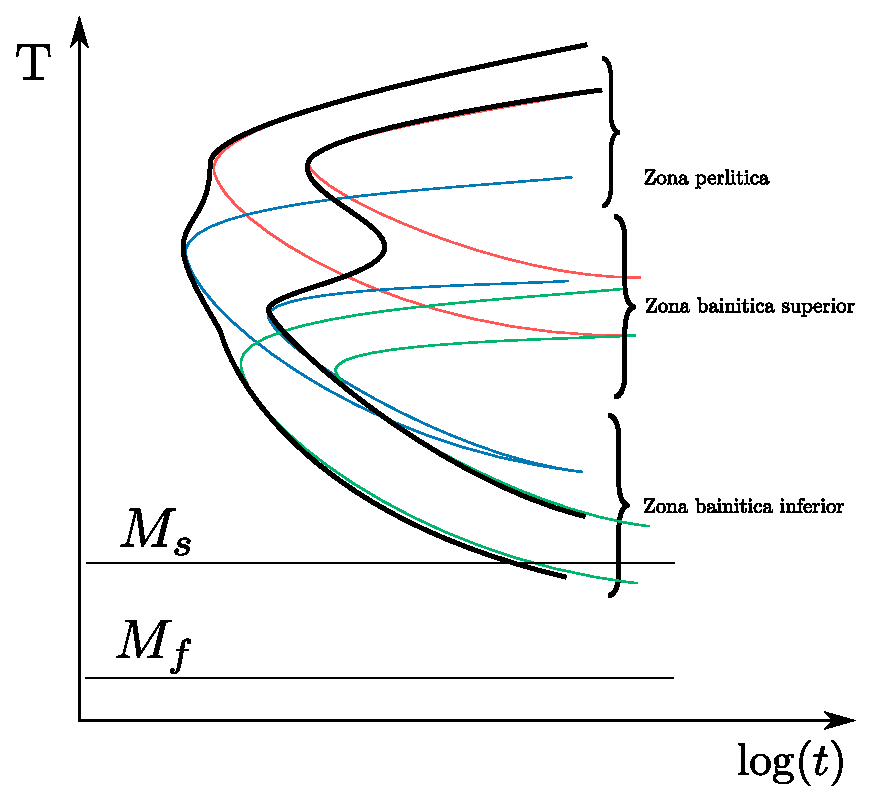
\includegraphics[width=0.7\textwidth]{fig/TTTsuperpuesta.eps}
    \caption{Superposición de curvas perlíticas (rojo) y bainíticas superior (azul) e inferior (verde).}
    \label{fig:TTTsuperpuestas}
\end{figure}

\section[Transformación de la austenita]{Variables que inciden en transformación de la austenita}
Dos variables que inciden en la cinética de estas transformaciones
\begin{itemize}
    \item El tamaño del grano austenítico
    \item La composición química de la austenita que se transforma.
\end{itemize}

Los borde de granos son los sitios de nucleación preferencial para las transformaciones perlítica y bainítica así como para la aparición de las fases proeutectoides ferrita y cementita. Por ende:
\begin{itemize}
    \item Mayor tamaño de grano \goright
    \item[\goright] Menor superficie total de bordes de granos \goright
    \item[\goright] Menor sitios de nucleación \goright
    \item[\goright] Transformaciones comienzan a mayores tiempos
\end{itemize}
\textbf{lo que implica que con mayor tamaño de grano las curvas se mueven a la derecha.}

La composición química juega un rol importante en el efecto sobre $\Delta G$ y $D_c$. Los elementos \textbf{gamágenos} hacen descender la energía libre de la austenita lo que reduce tanto la velocidad de nucleación como la de crecimiento. Los elementos alfágenos hacen subir la fuerza impulsora y en principio deberían acelerar las transformaciones, pero \hl{hacen exactamente lo contrario}.

Porqué sucede esto? En las palabras del profesor (resumidas): Durante la nucleación de ferrita en los borde de grano ocurre que los elementos \textbf{alfágenos} necesitan repartirse hacia la ferrita y los \textbf{gamágenos} necesitan concentrarse en la austenita. Ambos tienen un coeficiente de difusión mucho menor al del carbono y por eso se retrasan las transformaciones de fase.

Además! Los alfágenos son \textbf{formadores de carburos} lo que significa que se tienen que repartir hacia los mismos para que precipiten. Esto también retrasa las transformaciones que involucran precipitación de carburos. 

Algunos elementos simplemente retrasan la difusión del carbono, lo que también retrasa las transformaciones.

Efectos de elementos alfágenos:
\begin{itemize}
    \item Suben \Aone y \Athree (estabilización de ferrita [$\alpha$])
    \item Bajan \Bs, separando las curvas perlíticas y bainíticas
    \item Retrasan más la transformación ferrítica y perlítica que la bainítica. El Molibdeno acelera débilmente la transformación bainítica
    \item El Boro en diminutas cantidades (60ppm) provoca un fuerte retraso en la nucleación de la ferrita proeutectoide. De aquí surgen aceros de alta templabilidad.
\end{itemize}

Efectos de elementos gamágenos:
\begin{itemize}
    \item Bajan temperaturas \Aone, \Athree, \Bs y $M_s$
    \item Retrasan ambas transformaciones (perlita, bainita)
\end{itemize}

\section{Curvas CCT}
\textit{Continuous Cooling Transformation} son curvas representativas de las fases obtenidas a velocidad de enfriamiento constante. Cuando el enfriamiento es continuo desde el campo estable de $\gamma$, el tiempo de comienzo de la transformación no coincide con el que dice la curva TTT. Es porque la austenita pasa por un rango de T donde los periodos de incubación son grandes, de esta forma ``retrasando'' las curvas respecto las TTT.

\begin{figure}[htb!]
    \centering
    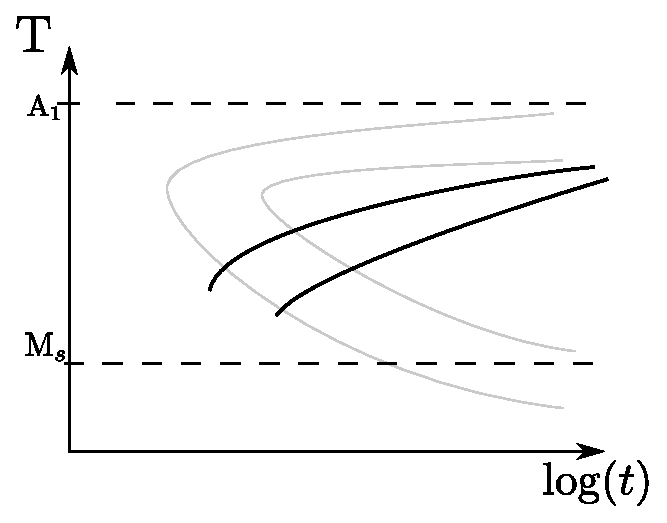
\includegraphics[width=0.8\textwidth]{fig/CCTeutect.eps}
    \caption{Curvas de enfriamiento continuo (CCT) para un acero \textbf{eutectoide}. CCT en negro, curvas TTT en gris claro.}
    \label{fig:CCTeutect}
\end{figure}

\subsection{CCT para un acero hipoeutectoide}
Las curvas de enfriamiento para un acero \textbf{hipoeutectoide} de la figura \ref{fig:CCThipo} pueden ceder las siguientes estructuras y microconstituyentes:\footnote{Tener en cuenta que las curvas rojas de la figura \ref{fig:CCThipo} se dibujan hasta donde haya austenita sin trasformar, es decir, el final de la curva esta donde $\gamma=0\%$.}


\begin{itemize}
    \item[Ciclo 1] Se obtiene ferrita de grano grueso y perlita gruesa en fracciones cercanas al equilibrio
    \item[Ciclo 2] Ferrita de grano mas fino que en el ciclo 1 y perlita fina. Perlita es diluida en ferrita que se encuentra presente en cantidades mayores a la de equilibrio. 
    \item[Ciclo 3] Ferrita, bainita y una fracción de Martensita que sale de la austenita que no se transformo al llegar a $M_s$ \footnote{La curva $M_s$ no es constante para todos los aceros. Si se tiene un acero hipereutectoide, al comenzar a formar bainita la concentración de carbono en la austenita sin transformar va aumentar, reduciendo asi $M_s$ a menor velocidad de transformación por ser un elemento gamágeno.}
    \item[Ciclo 4] Mínima velocidad de transformacion para lograr 100\% de martensita denominada \hl{Velocidad Critica de Temple}
\end{itemize}

\begin{figure}[htb!]
    \centering
    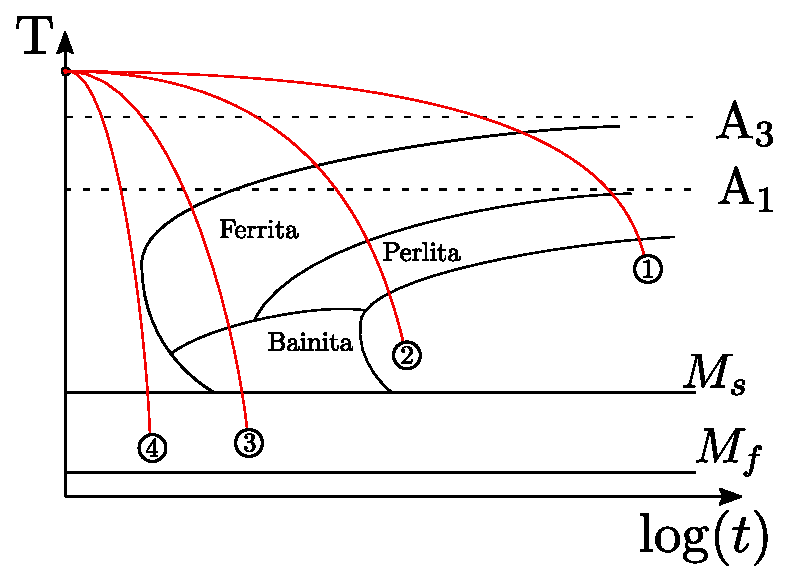
\includegraphics[width=0.7\textwidth]{fig/CCThipo.eps}
    \caption{Curvas de enfriamiento continuo (CCT) para un acero \textbf{hipoeutectoide}.}
    \label{fig:CCThipo}
\end{figure}

NOTA: La curva $M_s$ baja después de un tiempo dado!


\subsection{Variación de propiedades mecánicas con la velocidad de enfriamiento}
Aumentando la velocidad de enfriamiento de la austenita, las transformaciones ocurren en un rango de temperaturas más bajas, logrando microconstituyentes más finos que conlleva con un aumento de dureza y resistencia a la tracción. 

Las estructuras que surgen de un enfriamiento continuo son más complejas que las de transformaciones isotérmicas ya que al pasar por un rango más amplio de temperaturas de transformación se pueden obtener mezclas muy variadas de los microconstituyentes.